\newtheorem{myDef}{Definition}

\section{Formal Definitions}

\begin{myDef}
    Given a twice differentiable function $f(x)$ whose second derivative is continuous and some $N \in \mathbb{R}$, we define the \textbf{$N$-Units Away Curve} to be the collection of all points in $\mathbb{R}^2$ that are exactly $|N|$ units away from $y=f(x)$ along the normal line to $y=f(x)$ at some $x_o$. If $N$ is positive, include only those points that lie above the curve $y=f(x)$. If $N$ is negative, include only those points that lie below the curve.
\end{myDef}

\begin{myDef}
    \textbf{The ``Snipped'' $N$-Units Away Curve} is a function from $\mathbb{R}$ to $\mathbb{R}$ that we’ll denote $``f_N''(x)$ that can be created from the $N$-Units Away Curve by ``snipping'' off any of the divot triangles which occur every time the $N$-Units Away Curve crosses over itself. In the event that for a given value of $x$ multiple points on the N-Units Away Curve share that same $x$-value but have different y-values, we define $``f_N''(x)$ as taking on the $y$ value furthers from the original curve $y = f(x)$. Thus if $N$ is positive, it is the highest y value among them. If N is negative, it is the lowest.
\end{myDef}

Examples:

\begin{figure}[h!] 
  \label{formal-1} 
  \begin{minipage}[b]{0.45\linewidth}
    \centering
    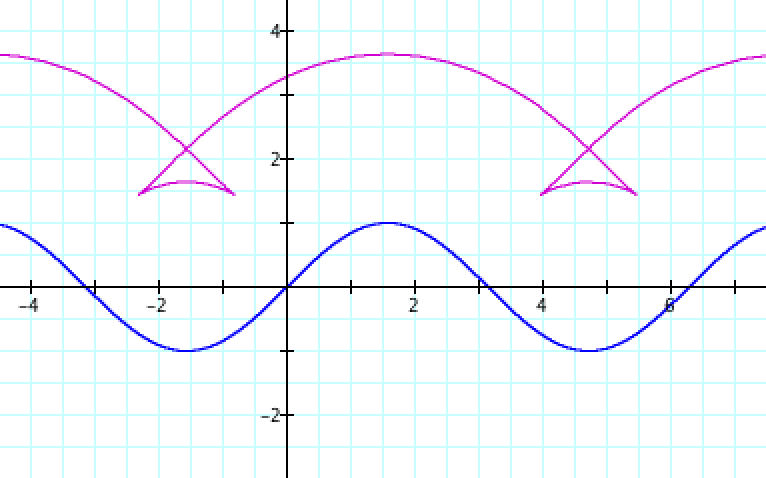
\includegraphics[width=\linewidth]{formal-definitions-img/Fig 13.png}
    \caption{$N$-Units Away Curve}
    \label{fig:fig13}
    \vspace{4ex}
  \end{minipage} % end 
  \begin{minipage}[b]{0.45\linewidth}
    \centering
    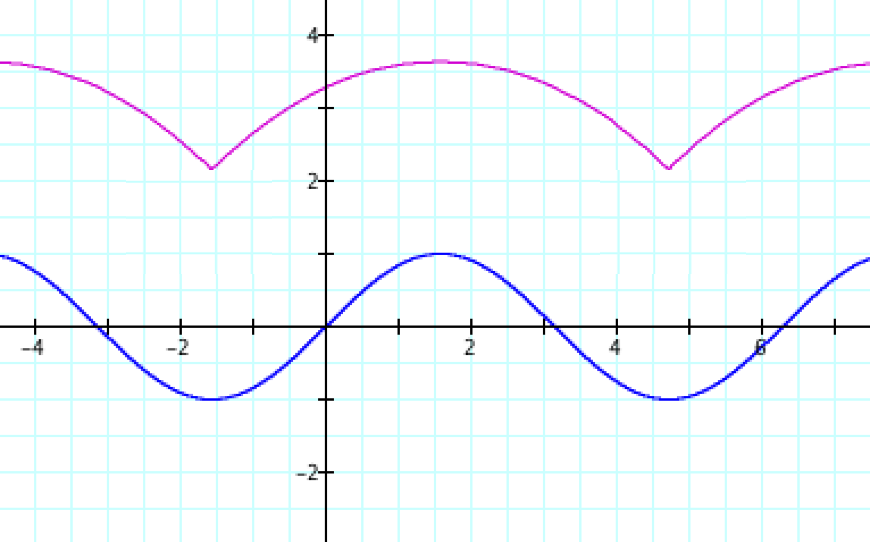
\includegraphics[width=\linewidth]{formal-definitions-img/Fig 14.png}
    \caption{``Snipped'' $N$-Units Away Curve}
    \label{fig:fig14}
    \vspace{4ex}
  \end{minipage} % end
\end{figure}

Just for the moment we'll take it as an assumption that $``f_N''(x)$ is defined on all of $\mathbb{R}$. We will return and establish this fact rigorously later on. Note that it was this ``snipped'' version of the $N$-Units Away Curve that my little kid self was drawing.